\documentclass{beamer}
\usetheme{Warsaw}

\usepackage[utf8]{inputenc}
\usepackage{amsmath}
\usepackage{amssymb}
\usepackage{graphicx}
\usepackage{booktabs}
\usepackage{graphicx}    % for \resizebox
\usepackage{array}       % for p{…} column types

\usepackage{adjustbox}
\title{The Deep Ritz Method }
\author{Heorhii Lopatin}
\date{\today}

\begin{document}

\begin{frame}
  \titlepage
\end{frame}

\begin{frame}
  \frametitle{Outline}
  \tableofcontents
\end{frame}

\section{Introduction}
\begin{frame}
  \frametitle{Solving PDEs}
  \begin{itemize}
    \item \textbf{Finite Difference Method}: Approximate derivatives on a grid.
    \item \textbf{Finite Element Method}: Divide the domain into elements and use variational methods.
  \end{itemize}
\end{frame}


\begin{frame}[c]{Comparison of Numerical Methods}  % [c] for vertical centering
% eliminate Beamer’s built‑in side margins
  \begin{adjustbox}{max width=\textwidth}
  \scriptsize
  \begin{table}[h]
  \begin{tabular}{|l|l|l|l|l|}
    \hline
    \textbf{Feature} 
      & \textbf{FEM} 
      & \textbf{FDM}  
      & \textbf{DRM} \\
    \hline
    Higher Dimensions 
      & Limited 
      & Limited 
      & Efficient \\
    \hline
    Adaptivity 
      & Limited 
      & Limited  
      & Naturally adaptive \\
    \hline
    Boundary Conditions 
      & Direct enforcement 
      & Direct enforcement 
      & Hard to enforce \\
    \hline
    Efficiency 
      & Moderate 
      & Moderate 
      & High on GPUs \\
    \hline
    Acc. w fewer parameters 
      & Moderate 
      & Moderate  
      & High \\
    \hline
  \end{tabular}
\end{adjustbox}
\end{table}
\end{frame}

\section{Some Machine Learning}
\begin{frame}
  \frametitle{Blocks}
  \begin{figure}
    \centering
    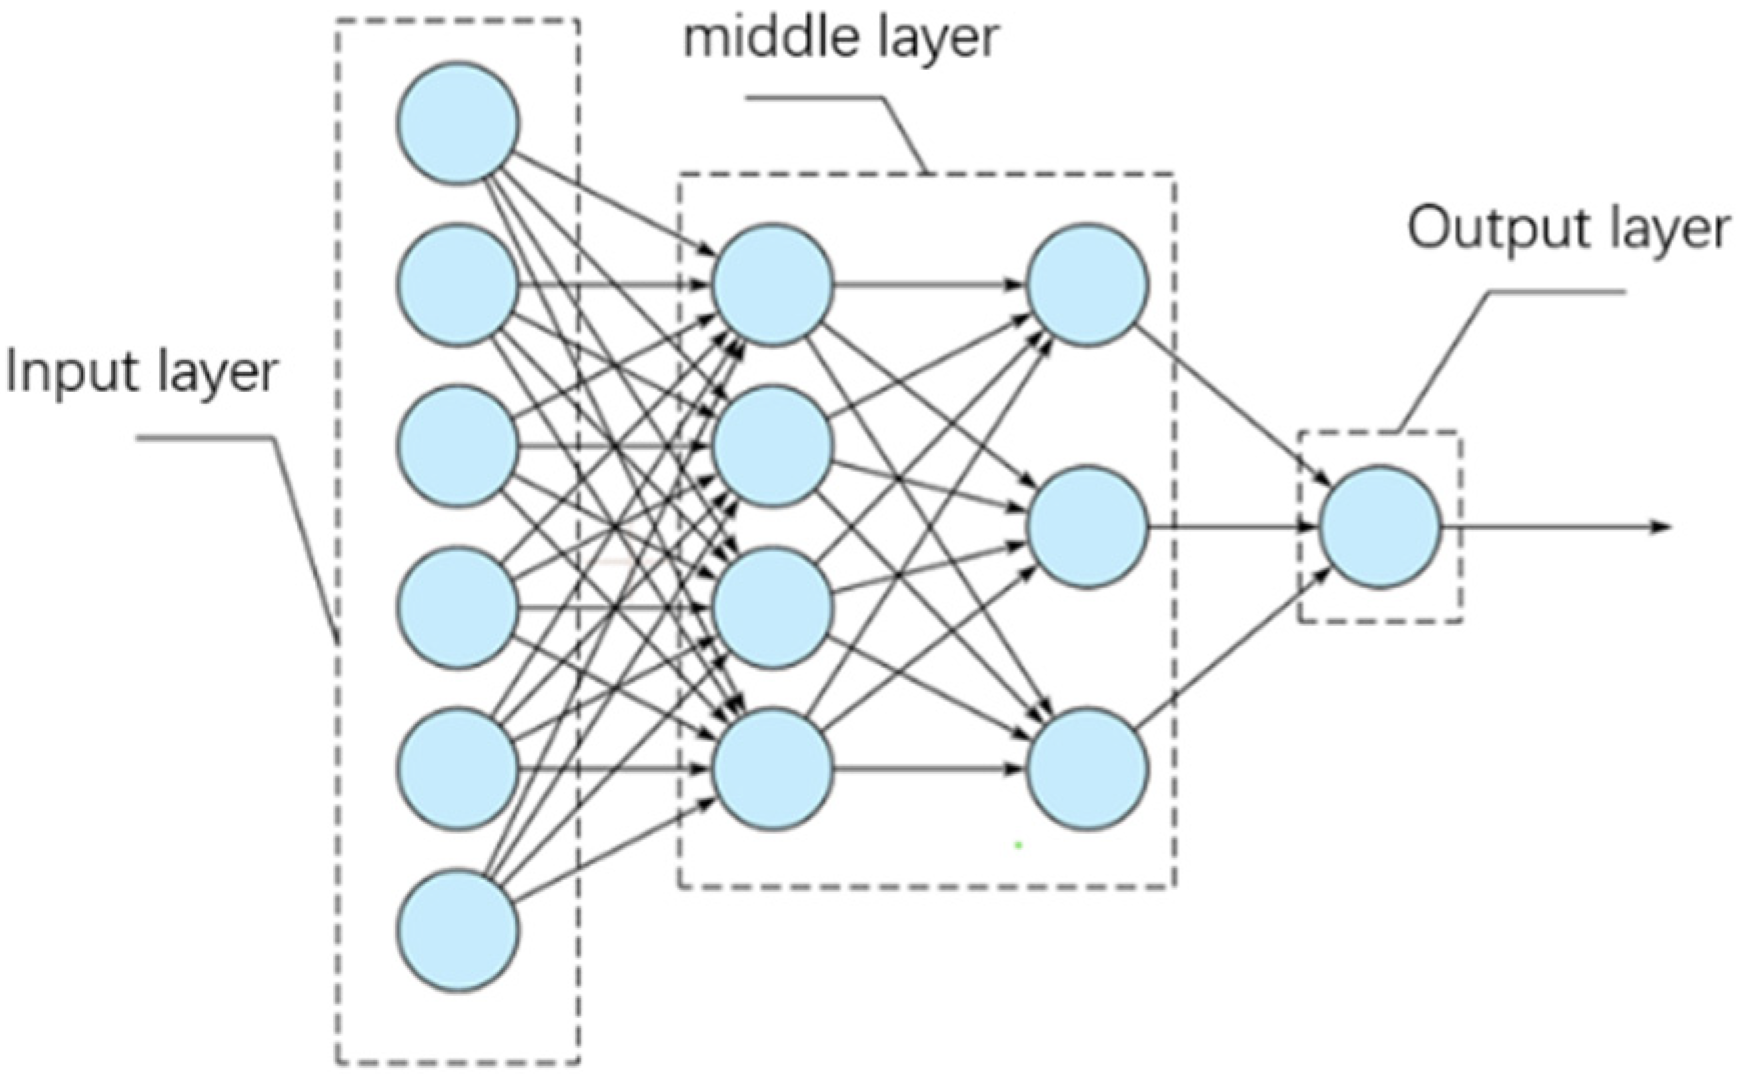
\includegraphics[width=0.8\textwidth]{block.png} % Placeholder - replace with an actual diagram
    \caption{www.mdpi.com}
  \end{figure}
''
\end{frame}
\begin{frame}
  \frametitle{Blocks}
  \begin{figure}
    \centering
    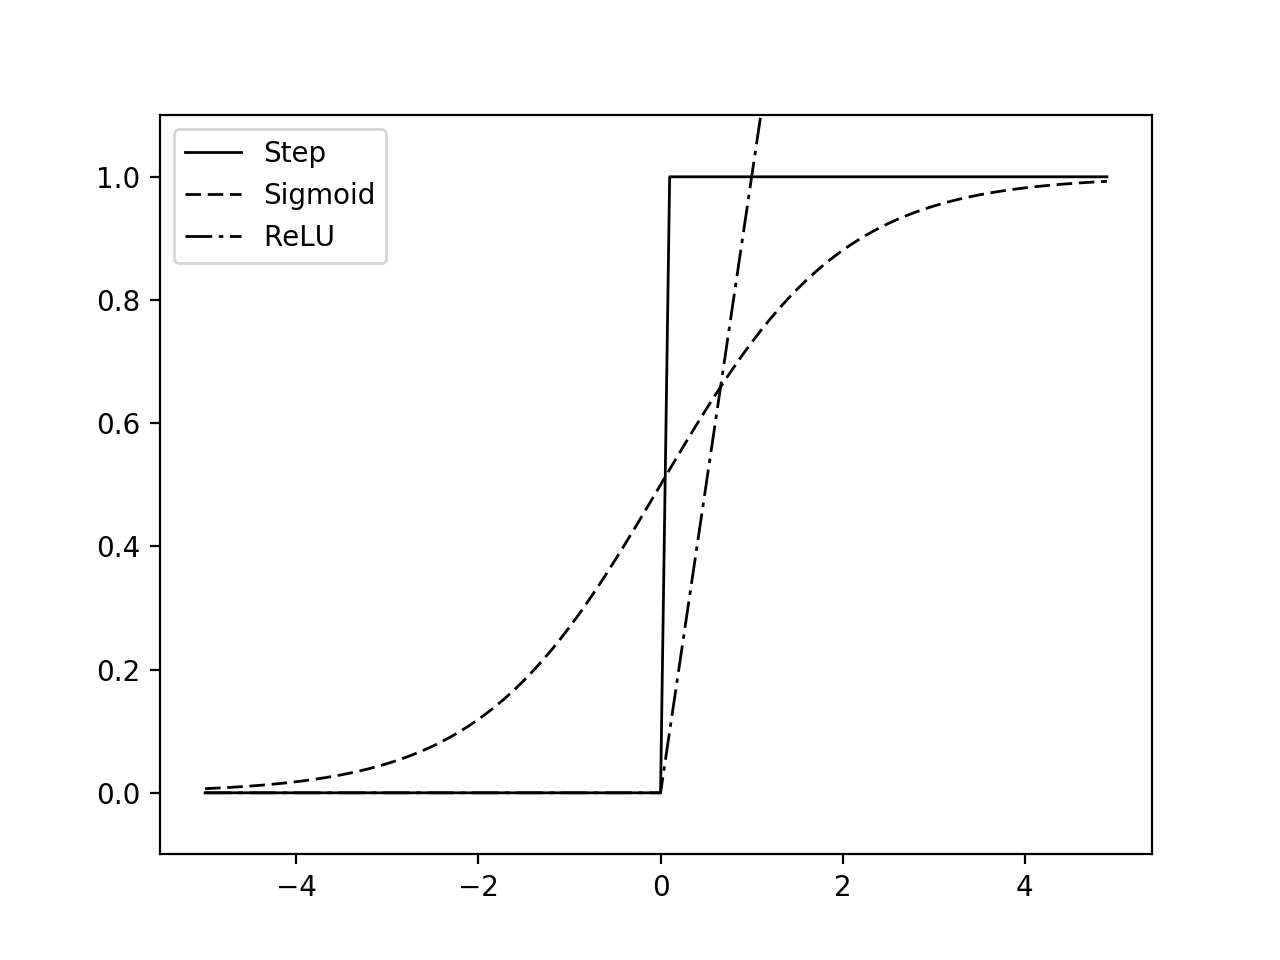
\includegraphics[width=0.7\textwidth]{function.png} % Placeholder - replace with an actual diagram
    \caption{schwalbe10.github.io}
  \end{figure}
\end{frame}

\begin{frame}
  \frametitle{Residual networks}
  \begin{figure}
    \centering
    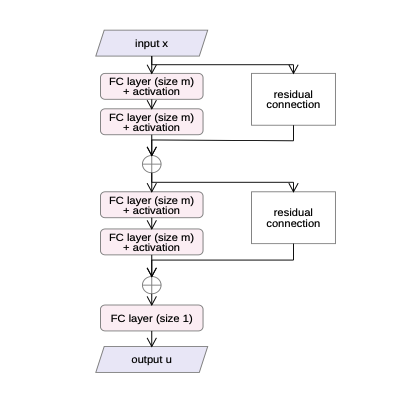
\includegraphics[width=0.7\textwidth]{dnn.png} % Placeholder - replace with an actual diagram
    \caption{[1]}
  \end{figure}
\end{frame}

\begin{frame}
  \frametitle{Value function}
            Score function $L(\theta)$ where $\theta$ are the parameters of the model.
            The goal of training is to find parameters $\theta^*$ that minimize this loss function.

\end{frame}

\begin{frame}

  \frametitle{Minimalization}
        \begin{itemize}
            \item \textbf{Gradient Descent (GD):} Iteratively update parameters in the opposite direction of the gradient of the loss function:
                $$\theta_{k+1} = \theta_k - \eta \nabla_{\theta} L(\theta_k)$$
                where $\eta$ is the learning rate. 
            \item \textbf{Backpropagation:} Algorithm used to efficiently compute the gradients $\nabla_{\theta} L(\theta_k)$ of the loss function with respect to the network parameters $\theta$. 
        \end{itemize}
\end{frame}

\begin{frame}
  \frametitle{Universal representation}
  \begin{itemize}
    \item The Sobolev norm:
    $$\|u\|_{H^1(\Omega)} = \left( \int_{\Omega} |u(x)|^2 dx + \int_{\Omega} |\nabla u(x)|^2 dx \right)^{1/2}$$
    The space $H^1_0(\Omega)$ refers to functions in $H^1(\Omega)$ that are zero on the boundary $\partial\Omega$. 
           \item Let $\Omega \subseteq \mathbb{R}^d$ be an open set and $u \in H^1_0(\Omega)$. Then for any $\epsilon > 0$, there exists a function $u_{\epsilon} \in H^1_0(\Omega)$ that can be expressed by a ReLU network of logarithmic depth on $d$ such that:
            $$\|u - u_{\epsilon}\|_{H^1(\Omega)} < \epsilon$$
          \end{itemize}
\end{frame}

\section{The Deep Ritz Method}
\begin{frame}
  \frametitle{Problems of Interest}
      \begin{itemize}
        \item \textbf{Poisson's Equation}: \( -\Delta u = f \) in \( \Omega \), with \( u = 0 \) on \( \partial\Omega \).
        \item \textbf{Schrödinger Equation}: \( -\Delta u + Vu = f \) in \( \Omega \), with appropriate boundary conditions.

        \item \textbf{Generalized Poisson's Equation}: -div$  \cdot \left( a(x) \nabla u(x) \right) + b(x) u(x) = f(x)$

      \end{itemize}
\end{frame}

\begin{frame}
  \frametitle{Variational Formulation}
  \begin{itemize}
    \item \textbf{Principle}:
      \begin{itemize}
        \item Convert PDEs into equivalent(?) minimization problems.
      \end{itemize}
    \item \textbf{Example}:
      \begin{itemize}
        \item For Poisson's equation, find \( u \in H^1_0(\Omega) \) minimizing:
          \[
          E(u) = \frac{1}{2} \int_\Omega |\nabla u|^2 dx - \int_\Omega fu dx
          \]
      \end{itemize}
    \item \textbf{Deep Ritz Method}:
      \begin{itemize}
        \item Approximate \( u \) with a neural network \( u_\theta \).
        \item Minimize \( E(u_\theta) \) with respect to \( \theta \).
      \end{itemize}
  \end{itemize}
\end{frame}

\begin{frame}
  \frametitle{Approximation of the Integral}
  \begin{itemize}
    \item \textbf{Challenge}:
      \begin{itemize}
        \item Computing integrals in high dimensions
      \end{itemize}
    \item \textbf{Solution}:
      \begin{itemize}
        \item Use Monte Carlo integration:
          \begin{itemize}
            \item Sample points \( \{x_i\} \) uniformly in \( \Omega \).
            \item Approximate integrals as averages over these samples.
          \end{itemize}
      \end{itemize}
  \end{itemize}
\end{frame}

\section{Theorems \& Experiments}
\begin{frame}
  \frametitle{Theorems}
  \begin{figure}
    \centering
    
\includegraphics[width=1.1\textwidth]{theorem.png} % Placeholder - replace with an actual diagram
    \caption{DEEP RITZ REVISITED: Johannes Muller, Marius Zeinhofer}
  \end{figure}
\end{frame}

\begin{frame}
  \frametitle{Theorems}
  \begin{figure}
    \centering
    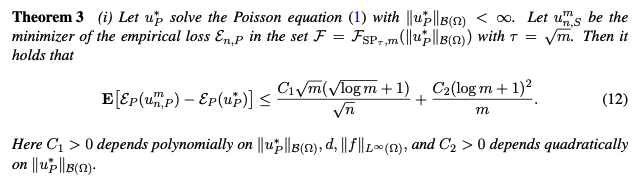
\includegraphics[width=\textwidth]{barron} % Placeholder - replace with an actual diagram
    \caption{A Priori Generalization Analysis of the Deep Ritz Method: Jianfeng, Yulong Lu, Min Wang}
  \end{figure}
\end{frame}
\begin{frame}
  \frametitle{Experiments}
  \begin{figure}
    \centering
    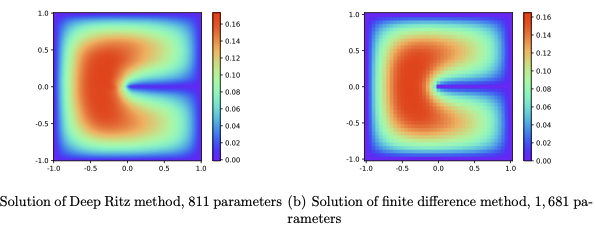
\includegraphics[width=\textwidth]{graph} % Placeholder - replace with an actual diagram
    \caption{The Deep Ritz method: Weinan E, Bing Yu}
  \end{figure}
\end{frame}

\end{document}
